%%%%%%%%%%%%%%%%%%%%%%% file template.tex %%%%%%%%%%%%%%%%%%%%%%%%%
%
% This is a general template file for the LaTeX package SVJour3
% for Springer journals.          Springer Heidelberg 2010/09/16
%
% Copy it to a new file with a new name and use it as the basis
% for your article. Delete % signs as needed.
%
% This template includes a few options for different layouts and
% content for various journals. Please consult a previous issue of
% your journal as needed.
%
%%%%%%%%%%%%%%%%%%%%%%%%%%%%%%%%%%%%%%%%%%%%%%%%%%%%%%%%%%%%%%%%%%%
%
% First comes an example EPS file -- just ignore it and
% proceed on the \documentclass line
% your LaTeX will extract the file if required
\begin{filecontents*}{example.eps}
%!PS-Adobe-3.0 EPSF-3.0
%%BoundingBox: 19 19 221 221
%%CreationDate: Mon Sep 29 1997
%%Creator: programmed by hand (JK)
%%EndComments
gsave
newpath
  20 20 moveto
  20 220 lineto
  220 220 lineto
  220 20 lineto
closepath
2 setlinewidth
gsave
  .4 setgray fill
grestore
stroke
grestore
\end{filecontents*}
%
\RequirePackage{fix-cm}
%
%\documentclass{svjour3}                     % onecolumn (standard format)
%\documentclass[smallcondensed]{svjour3}     % onecolumn (ditto)
%\documentclass[smallextended]{svjour3}       % onecolumn (second format)
\documentclass[twocolumn]{svjour3}          % twocolumn
%
\smartqed  % flush right qed marks, e.g. at end of proof
%
\usepackage{graphicx}
\usepackage{amsmath}
\usepackage{amsfonts}
\usepackage{algorithm}
\usepackage{color}
%
\usepackage{mathptmx}      % use Times fonts if available on your TeX system
%\usepackage{cite}
%\usepackage{url}
\usepackage{hyperref}
% insert here the call for the packages your document requires
%\usepackage{latexsym}
% etc.
%
% please place your own definitions here and don't use \def but
% \newcommand{}{}
%\newcommand{\cxj}[1]{\textcolor[rgb]{1.00,0.00,0.00}{(cxj: #1)}}
%highlight the modification
\newcommand{\mdf}[1]{\textcolor[rgb]{1.00,0.00,1.00}{#1}}
%\newcommand{\hsy}[1]{\textcolor[rgb]{0.44,0.67,0.22}{(hsy: #1)}}
%\newcommand{\confirm}[1]{\textcolor[rgb]{0.00,1.00,1.00}{#1}}
\newcommand{\vb}[1]{\mathbf{#1}}
\newcommand{\defV}{\mathcal{V}}
\newcommand{\defZ}{\mathcal{Z}}
\newcommand{\comments}[1]{}
%
% Insert the name of "your journal" with
% \journalname{myjournal}
%
\begin{document}

\title{Point Sets Joint Registration and Co-segmentation%\thanks{Grants or other notes
%about the article that should go on the front page should be
%placed here. General acknowledgments should be placed at the end of the article.}
}
\subtitle{}

%\titlerunning{Short form of title}        % if too long for running head

\author{Siyu Hu         \and
        Xuejin Chen \and
        Xin Tong
}

%\authorrunning{Short form of author list} % if too long for running head

\institute{Siyu Hu \at
	Dept. of Electronic Engineering and Information Science
	University of Science and Technology of China\\
              \email{sy891228@mail.ustc.edu.cn}           %  \\
%             \emph{Present address:} of F. Author  %  if needed
           \and
           Xuejin Chen \at
           Dept. of Electronic Engineering and Information Science
           University of Science and Technology of China\\
           \email{xjchen99@ustc.edu.cn}
           \and
           Xin Tong \at
           Microsoft Research Asia\\
           \email{xtong@microsoft.com}
}

\date{Received: date / Accepted: date}
% The correct dates will be entered by the editor


\maketitle

\begin{abstract}
We present a novel approach of joint registration and co-segmentation for point sets where objects move in different ways. 
Considering the joint registration and co-segmentation as two problems heavily entangled with each other, we represent the input point sets as samples from a generative model and bring up with a novel formulation based on Gaussian mixture model. %
By maximizing the posterior probability of the samples, we gradually recover the latent object models as well as an object-level segmentation, and simultaneously align the segmented points to the latent object models. 
%
Along with the formulation, we design an interactive tool that helps users intuitively intervene the process to optimize the registration and segmentation result. 
%
The experiment results on a group of synthetic and scanned point clouds demonstrate that our method is powerful and effective for joint registration and co-segmentation on point sets of multiple objects. 
\keywords{Point Cloud \and Registration \and Co-segmentation}
% \PACS{PACS code1 \and PACS code2 \and more}
% \subclass{MSC code1 \and MSC code2 \and more}
\end{abstract}

\section{Introduction}
\label{sec:intro}
\mdf{In this paper, we present a new method to solve the object-level joint registration and co-segmentation problem. This problem originates from our attempt to build databases from scanned data.} \hsy{One reviewer said we should state this at the beginning of the introduction, he didn't understand our motivation until the late of introduction}
Many research projects and applications of indoor scenes require segmented, and even annotated 3D databases~\cite{SearchClassify,SceneFromExample,Fisher:2012:ESO:2366145.2366154,Chen:2014:ASM:2661229.2661239,Fisher:ActivityCentricSceneSynthesis}).
%
One way to build such a database is to interactively compose scenes using 3D object models, resulting in scenes with object segmentation and annotation naturally available, or to manually segment and annotate existing 3D scenes. 
%
This procedure can be tedious and time consuming, despite many efforts of improving the interaction experience~\cite{Merrell:2011:IFL:2010324.1964982, Xu:2013:SSC:2461912.2461968}.
%
Another way is to automatically generate scenes from 3D shape models according to images~\cite{Liu2015Model,Chen:2014:ASM:2661229.2661239}. 
%
In these methods, a retrieval procedure is usually needed and inevitably limit the result to a certain set of 3D models despite the actual 3D model in the input images.

Generating scene models directly from captured point clouds will significantly facilitate dataset construction and \mdf{increase} the dataset variety.
%
One of the major gaps between the required dataset and the available scene capturing frameworks~\cite{KinectFusion, dai2016bundlefusion} is the generic object-level segmentation. 
%
A generic object-level segmentation is not an equivalence of multi-label classification problem since it is not limited to a fixed number of objects in different scenes. 
%
Existing approaches for segmenting scanned 3D data require additional knowledge, such as the block-based stability~\cite{3DReasoningfromBlockstoStability}, or the motion consistency of rigid objects~\cite{Xu:2015:ACS:2816795.2818075}.  
%
%\cite{Xu:2015:ACS:2816795.2818075} proposes a practical and rather complete framework to close the gap between the required data set and available scene capturing method. 
%
%One of the observation in \cite{Xu:2015:ACS:2816795.2818075} is that the motion consistency of rigid object can serve as a strong evidence of general objectness.
While they employ a robot to do proactive push and use the movement tracking to verify and iteratively improve their object level segmentation result, \mdf{it remains significantly} challenging to recover the motion consistency in a \mdf{non-invasive} way.
\hsy{Without robot, our method is more tedious, since we need to schedule scanning every day.}


In this paper, we explore the motion consistency of rigid objects in a different aspect.
%
While the motion consistency of objects in indoor scenes is naturally revealed by human activities along the time, we hope to segment the objects in a scene from the scanned point clouds at different times. 
%
With respect to this idea, we are facing the choice of scanning schemes. 
%
One way is to record the change of the scene along with human activities.
Another option is to schedule a periodic sweep that only records the result of human activities but avoids the instants of human motion. 
%
The main challenge brought in by the second scheme is that we may not be able to solve the object correspondence by a local search due to the sparse sampling over time.
However, the very same challenge exists in the first scheme due to the occlusion caused by human bodies, not to mention other additional process (e.g. tracking with severe occlusions) needed for human bodies.
%
Therefore, we choose the second scheme.
\cxj{What is the advantage of the second scheme?} \hsy{Both schemes are difficult. We simply choose the less difficult one. The second scheme simply has less disadvantage.}
%
With the second scanning scheme, our original intention of building 3D scene datasets from canned data leads us to the problem of coupled joint registration and co-segmentation.


In this problem, registration and segmentation are entangled in each other. 
%
On one hand, the segmentation depends on the registration to connect the point clouds into series of rigid movement so that the object-level segmentation can be done based on the motion consistency. On the other hand, the registration depends on the segmentation to break the problem into a series of rigid joint registration instead of a joint registration with non-coherent point drift.
Non-coherent point drift means that a pair of points is close to each other in one point set, but their corresponding pair of points in another point set is far from each other. 
%
This happens when this pair of points actually belong to different objects.


We employ a group of Gaussian mixture models and each of these Gaussian mixture models represents a potential object. 
This model unentangle \cxj{Where do you find the word "unentangle"? did you create it?} \hsy{As verbs the difference between untangle and unentangle is that untangle is to remove tangles or knots while unentangle is to reverse the process of entanglement. Disentangle is to free something from entanglement.} the registration and segmentation in the way that the segmentation can be done by evaluate the probability of points belongs to the Gaussian mixture models and the registration can be done by evaluate rigid registration against each Gaussain mixture models.


In summary our work makes following contributions: 
\begin{enumerate}
	\item To the best of our knowledge, we first put forward the problem of joint registration and co-segmentation of point sets.
	
	\item We propose a generative model to simultaneously solve the joint registration and co-segmentation of point sets.
	
	\item We design a practical tool for efficient joint registration and co-segmentation based on the generative model. 
	
\end{enumerate}


\section{Related Work}
\label{sec:rw}
In this section we explain how our work is related to the previous work on point set processing and how we draw experiences from these methods. 

%\subsection{Point Set Registration with GMM Representation}
%\label{subsec:gmmreg}
\noindent{\textbf{Point Set Registration with GMM Representation.}}
There is a series of approaches that use Gaussian mixture model as \mdf{the} representation for point set registration problems \cxj{due to its general ability of representing point sets for both rigid and non-rigid registation}.
%
%
A \mdf{comprehensive} survey about approaches for point set registration using Gaussian mixture models can be found in \cite{GMM_PAMI}. 
They also present a unified framework for rigid and nonrigid registration problems. 
%
These methods select one of the point sets as the ``model'' and align other point sets with this \mdf{template}. \cxj{Is it better to use "template" than ``model''?} 
%
Myroeko and Song consider the registration of two point sets as a probability density estimation problem, and use Gaussian mixture model to represent the geometry and force the GMM centroids to move coherently as a group to preserve the topological structure of the point sets \cite{CPD}. This method is applicable to both rigid registration and non-rigid registration. \cxj{Does this method treat one point set as the template?}
%
As we highlighted in Sec.~\ref{sec:intro}, our problem is different from the non-rigid registration while the point drift is non-coherent in our \mdf{problem}.
%
Unlike these works, \cite{Evangelidis2014} treats all point sets equally.
They are all realizations of a Gaussian mixture model and the registration is cast into a clustering problem. 
A recent method pushes this idea to the application on a large scale dataset~\cite{GOGMA}. 
Comparing to these methods, our method can be seen as an extension of the formulation of \cite{Evangelidis2014} to simultaneously handle joint registration and co-segmentation. 
\cxj{It should not be a simple extension. You should highlight what is the most challeging part we solved compared with others. I would say: } \mdf{In comparison, we employ the same GMM representation of object models while we formulate the non-coherent point drift as .....  }

%\subsection{Image segmentation and co-segmentation}
%\label{subsec:coseg}
\noindent{\textbf{Image segmentation and co-segmentation}}
%
An influential work for interactive image segmentation is GrabCut~\cite{grabcut}. It uses two Gaussian mixture models, one for foreground and the other for background. 
To initialize these two Gaussian mixture models, a rectangle is manually placed to contain the foreground. 
Our design of interaction draws on the \mdf{experience} from \cite{grabcut}. 
%
The difference is that our interaction is designed for 3D space and can handle multi-object segmentation rather than foreground-background segmentation. 
%
\cite{Taniai_2016_CVPR} jointly recovers co-segmentation and dense per-pixel correspondences in two images. 
Its co-segmentation is limited to foreground-background segmentation. Our work solves a similar problem for multiple 3D point sets. 
\cxj{There are many image co-segmentation papers. If you want to discuss it, you should discuss more. }

\noindent{\textbf{Segmentation from Motion.}}
The idea that motion can be a strong hint for segmentation is used in many works.
\cite{Xu:2015:ACS:2816795.2818075} employs a robot to do proactive push and track the motion to learn object segmentation. 
\cite{unsupervisededge} exploits the motion in a video and uses the motion edges as the training data to learn an edge detector for image \cxj{use 'an image' or 'images'}. 
These methods lean on the motion that is continuous in time and can be tracked. Our method can handle motion that is not continuous in time.

\noindent{\textbf{3D Object Recognition based on Correspondence Grouping.}}
By allowing interactively input \mdf{the scene layout}, the joint registration and co-segmentation problem can be treated as a series of 3D object recognition problem in point sets. Our method should be classified as one of the correspondence grouping method. Comparing to previous methods \cxj{that uses ...}~\cite{hough,LOF}, our method simultaneously solve\mdf{s} the problem for multiple target models in multiple scenes.

\section{Method Overview}
\label{sec:method}
\subsection{Problem Statement}
Given series of point sets which record the same group of rigid indoor objects with different layout. We intend to samutaneously partition the point sets into objects and align the points of same object to recover layouts for corresponding object. Figure~\ref{fig:teaser} shows an example of input point clouds set.
\subsection{Basic Formulation}
To simutaneously model the joint registration and co-segmentation,  we come up with a generative model as follows:
\begin{equation}
\label{equ:model}
P(v_{mi})=\sum^{K_n}_{k=1}p_kN(v_{mi}|\phi_{mn}(x_k),\Sigma_k)
\end{equation}
which treat the i-th observed point $v_{mi}$ from the m-th point set as a sample point generated by one of $N$ object models.
We can define:\\
$$\Theta=\{\{p_k,x_k,\Sigma_k\}_{k=1}^{\sum{K_n}},\{\phi_{mn}\}_{m=1,n=1}^{MN}\}$$
as the parameter set of the generative model.\\
$p_k$ is the weight of the k-th Gaussian.\\
$x_k$ is the center of the k-th Gaussian.\\
$\Sigma_k$ is the standard deviation of the k-th Gaussian.\\
There are $K_{all}=\sum{K_n}$ Gaussian models in total and among them $K_n$ Gaussian models are treated as a group to represent n-th object.\\
$V$ is the set of M input point sets.\\
$v_{mi}$ is the i-th point of the m-th point cloud.\\
$\{\phi_{mn}\}$ are the functions of rigid transformation that transform the n-th group of gaussian centroids (representing the n-th object ) to the space of m-th input point sets.\\ 
Each object model is represented by a group of $K_n$ gaussian models.\\
Our goal of optimization is to maximize the probability of observed input sets sampled from the latent model.This problem can be solved in the framework of expectation-maximization. In particular, we bring in a latent parameter\\
$$Z=\{z_{mn}|m=1...M,n=1...N_m\}$$
such that $z_{mn}=k(k=1...\sum{K_n})$ assigns the observed point $v_{mi}$ to the k-th component of Gaussian mixture model. We aim to maximize the expected complete-data log-likelihood:
\begin{equation}
\label{equ:obj0}
f(\Theta|V,Z)=\mathbb{E}_Z[\ln P(V,Z;\Theta)|V]
\end{equation}
The object can be written as:
\begin{equation}
\label{equ:obj1}
\Theta=\arg\max{\sum_ZP(Z|V,\Theta)\ln{P(V,Z;\Theta)}}
\end{equation}
Such formulation can be seen as an adaption of joint registration formulation in \cite{Evangelidis2014}, upon which we seperate Gaussian models into groups to express multiple objects and the latent parameter  $Z$ that assign observed points to gaussian models can naturally indicate the object level segmentation.\\
By the asssumption of independent and identically distributed of input points, we can write the objective to:
\begin{equation}
\label{equ:obj2}
\Theta=\arg\max\sum_{mik}\alpha_{mik}(\ln p_k + \ln P(v_{mi}|z_{mi}=k;\Theta))
\end{equation}
where $\alpha_{mik} = P( z_{mi} = k | v_{mi} ; \Theta )$\\
By bringing in equation \ref{equ:model} and ingnoring constant terms, we can rewrite the objective as:
\begin{equation}
\label{equ:obj3}
\Theta=\arg\max\sum_{mik}\alpha_{mik}(||v_{mi}-\phi_{mn}(x_k)||_{\Sigma_k}^2 + \ln |\Sigma_k| - 2\ln p_k)
\end{equation}
where the $|\cdot|$ denotes the determinant and $||x||_A^2=x^TA^{-1}x$. It is predefined that $x_k$ is one of the gaussian centroid used to represent n-th object, which is why we apply transformation $\phi_{mn}$ on to the $x_k$. For the convenience of computation, we restrict the model to isotropic covariances, i.e.,$\Sigma_k=\sigma^2I$ and $I$ is the identity matrix.\\
Now, we can optimize this through iterating between estimating $\alpha_{mik}$ (Expectation-step) and maximizing $f(\Theta|V,Z)$ sequentially with respect to each parameters in $\Theta$ (Maximization-steps).
These steps are:\\
\textbf{E-step}:
this step estimates the posterior probability $\alpha_{mik}$ of $v_{mi}$ to be a point generated by the k-th Gaussian model.\\
\begin{equation}
\label{equ:estep}
\alpha_{mik}=\frac{p_k\sigma_k^{-3}exp(-\frac{1}{2\sigma_k^2}||v_{mi}-\phi_{mn}(x_k)||^2)}{\sum_s^{K_{all}}p_s\sigma_s^{-3}exp(-\frac{1}{2\sigma_s^2}||v_{mi}-\phi_{mn}(x_s)||^2)}
\end{equation}
\textbf{M-step-a}:this step update the transformations $\phi_{mn}$ that maximize $f(\Theta)$, given instant values for $\alpha_{mik}$, $x_k$, $\sigma_k$. We only consider rigid transformations, making  $\phi_{mn}(x)=R_{mn}x+t_{mn}$. The maximizer $R_{mn}^*,t_{mn}^*$  of $f(\Theta)$ is the same with the minimizers of the following constrained optimization problems:\\
\begin{equation}
\left\{
\begin{array}{rcl}
\min_{R_{mn},t_{mn}}&      &||(W_{mn}-R_{mn}X_n-t_{mn}\mathbf{e}^T)\Lambda_{mn}||_F^2\\
s.t.&      &R_{mn}^TR_{mn}=I, |R_{mn}|=1\\
\end{array} \right.
\end{equation}
where $\Lambda_{mn}$ is $K_n \times K_n$ diagonal matrix with elements $\lambda_{mnk}=\frac{1}{\sigma_k}\sqrt{\sum_i^{I_{m}}\alpha_{mik}}$,$I_m$ is the number of point for the m-th input point set, $X_n = [x_1,x_2,....,x_{K_n}]$ is the matrix stacked by the centroids of gaussian models that are predefined to represent the n-th object. $\mathbf{e}^T$ is a vector of ones, $||\cdot||_F$ denotes the Frobenius norm, and $W_{mn}=[w_{m1},w_{m2},...,w_{mk},...,w_{mK_n}]$, in which $w_{mk}$ is a weighted point as:\\
\begin{equation}
w_{mk}=\frac{\sum_{i=1}^{I_m}\alpha_{mik}v_{mi}}{\sum_{i=1}^{I_m}\alpha_{mik}}
\end{equation}
This problem have a similar solution of in \cite{Evangelidis2014}. The only difference is that we are estimating the transformation from latent models to the input point sets, since there are multiple group of $x_k$ corresponding to multiple objects in our latent model. The optimal can be given by:\\
\begin{equation}
R_{mn}^*=U_{mn}C_{mn}V_{mn}^T
\end{equation}
\begin{equation}
t_{mn}^*=\frac{1}{tr(\Lambda_{mn}^2)}(W_{mn}-R_{mn}X_n)\Lambda_{mn}^2\mathbf{e}
\end{equation}
where $[U_{mn},S,V_{mn}]=svd( W_{mn}\Lambda_{mn}P_{mn}\Lambda_{mn}X_{mn}^T )$ and $P_{mn}=I-\frac{\Lambda_{mn}\mathbf{e}(\Lambda_{mn}\mathbf{e})^T}{(\Lambda_{mn}\mathbf{e})^T\Lambda_{mn}\mathbf{e}}$,$I$ is identity matrix. $C_{mn}=diag(1,1,|U_{mn}||V_{mn}|)$.\\
\textbf{M-step-b}: this step we update the parameters related to the Gaussian mixture model. 
\begin{equation}
x_k^*=\frac{\sum_{m=1}^M\sum_{i=1}^{I_m}\alpha_{mik}(R_{mn}^{-1}v_{mi}-t_{mn})}{\sum_{m=1}^M\sum_{i=1}^{I_m}\alpha_{mik}}
\end{equation}
where $x_k$ is one of the Gaussian centroids that is predefined to represent n-th object. 
\begin{equation}
\sigma_k^{*2}=\frac{\sum_{m=1}^M\sum_{i=1}^{I_m}\alpha_{mik}||(v_{mi}-t_{mn}-R_{mn}^*x_k^*)||_2^2}{3\sum_{m=1}^M\sum_{i=1}^{I_m}\alpha_{mik}}
\end{equation}
\begin{equation}
p_k^*=\frac{\sum_{m,i}\alpha_{mik}}{M}
\end{equation}
\subsection{Bilateral Formulation}
When considering features, we can add bilateral terms into the generative model.
\begin{equation}
P(v_{mi},f_{mi})=\sum^{K_n}_{k=1}p_kN(v_{mi}|\phi_{mn}(xv_k),\sigma v_k)N(f_{mi}|xf_k,\sigma v_f)
\end{equation}
we measure the feature difference by a gaussian with diagnal $\Sigma$.
\subsection{Interaction Design}
Unfortunately, there are serveral parameters that can not be easily initialized in our formulation . In this subsection we first introduce our design of interaction, which is intuitive for users to input the semantic prior this way. We then explain how we can easily initlialize those parameters for our optimization based on the manual input.\\
As demonstrated in Figure~\ref{fig:interact}, we let user choose one of the point sets and placing and editing boxes in it to indicate the layout for this point set. From this, we can easily initialize the total number of objects $N$ and determine $\{K_n\}$ which is the numbers of Gaussian mixture models used to represent each object.
\begin{figure}[htb]
	\centering
	\includegraphics[width=.3\linewidth]{images/interact01.png}
	\includegraphics[width=.3\linewidth]{images/interact02.png}
	\includegraphics[width=.3\linewidth]{images/interact03.png}
	\includegraphics[width=.3\linewidth]{images/interact04.png}
	\includegraphics[width=.3\linewidth]{images/interact05.png}
	\includegraphics[width=.3\linewidth]{images/interact06.png}
	\caption{\label{fig:interact}
		From the first to the nineth, the nine images show the procedure of interaction:
		the user pick one point set and place boxes in it to indicate the layout for this point set. The box in white is the box currently under editing. The boxes in other colors are boxes placed to represent object layouts. One color represent one object. The interaction allows multiple boxes to represent same object.(e.g. the desk is represented by three boxes in same color)}
\end{figure}
These two paremeters are difficult to be initialized without semantic prior, but with the input of the users we can naturally initialize the $N$ as the number of different color label and the ${K_n}$ as 
\begin{equation}
K_n=\frac{V_n}{\sum V_n}K_{all}
\end{equation}
in which the $V_n$ represent the total volume of the boxes in the n-th color and the $K_{all}$ is initialized as $K_{all}=0.5*median(I_m)$ and $\{I_m\}$ are point numbers of $M$ input point set. This is an emperical choice borrowed from \cite{Evangelidis2014}.\\
The expectation maximizaton framework is easily converge to a local optimal. To cope with this problem we further use this interaction as a soft constraint to guide the optimization. Such constraint is done by simply altering the posterior probability $\alpha_{mik}$ as\\
\begin{equation}
\alpha_{mik}^*=\frac{\alpha_{mik}\beta_{mik}}{\sum_{i,k}\alpha_{mik}\beta_{mik}}
\end{equation}
where the $\beta_{mik}$ is the prior probability according to the boxes. It is defined as:\\
\begin{equation}
\beta_{mik}=\left\{
\begin{array}{rcl}
1&      & v_{mi} \in B_n\\
\exp(-\frac{\min_{v_{mj}}|| v_{mi} - v_{mj} ||_2^2  )}{C})&      &v_{mi} \notin B_n~and~v_{mj} \in B_n\\
\end{array} \right.
\end{equation}
where the $B_n$ is a point set that is enclosed by the boxes used to represent the layout of n-th object. The k-th Gaussian model is predefined to be one of the Gaussians used to represent n-th object. $\min_{v_{mj}}|| v_{mi} - v_{mj} ||_2^2$ is actually the squared euclidean distance from point $v_{mi}$ to the point set $B_n$, as we define the distance from a point to a point set as the minimum distance from the point to any point inside the point set. 



\section{Initialization and Optimization}
\label{sec:imp}
In this section, we summarize the entire framework for our algorithm and explain how do we intialize the parameters and guide the optimization with interaction.  
%
Based on our formulation in Sec.~\ref{sec:method}, our algorithm can be summarized as in Algorithm \ref{alg:jrcs}.
\begin{algorithm}[htb]
	\caption{Joint Registration and Co-segmentation (JRCS)}
	\label{alg:jrcs}
	\textbf{Input:}~~\\
	$\{\vb{V}_m\}$:$M$ 3D point sets\\
	$\Theta^0$:Initial parameters\\
	$\{\beta_{ik}\}_{m}$:layout based prior\\
	\textbf{Output:}~~\\
	$\Theta^q$:Final parameters~~
	\begin{enumerate}
		\item $q\leftarrow1$
		\item \textbf{repeat}
		\item E-step: Use $\Theta^{q-1}$ to estimate $\alpha_{mik}^q$ according to Eq.~(\ref{equ:estep}) (use Eq.~(\ref{equ:bestep}) for a bilateral formulation);
		\item Alter $\alpha_{mik}^q$ with $\{\beta_{ik}\}_{m}$ according to Eq.~(\ref{equ:alteralpha});
		\item M-step-a: use $\alpha^q_{mik}$, $\mathbf x^{q-1}_k$ to estimate $\{\mathbf{R}_{mn}^q\}$ and $\{\mathbf t_{mn}^q\}$ according to Eqs.~(\ref{equ:updateR})(\ref{equ:updatet});
		\item M-step-b: use $\alpha^q_{mik}$, $\{\mathbf{R}_{mn}^q\}$ and $\{\mathbf{t}_{mn}^q\}$ to update other parameters for Gaussian models according to Eqs.~ (\ref{equ:updatexk})(\ref{equ:updatesigma})(\ref{equ:updatepk})(\ref{equ:updatey})  (or use Eqs.~ (\ref{equ:updatefk})(\ref{equ:updatefsigma}) for a bilateral formulation);
		\item $q \leftarrow q+1$
		\item \textbf{until} Convergence \cxj{what is the convergence conditions?}
		\item \textbf{return} $\Theta^q$
	\end{enumerate}
\end{algorithm}

\subsection{Interaction}
\label{sec:imp:interact}
Unfortunately, there are a large number of parameters that can not be easily initialized in our formulation. 
%
In this subsection we first introduce our design of interaction, which is intuitive for users to input the semantic prior this way. We then explain how we can easily initialize those parameters for our optimization based on the manual input.


As demonstrated in Figure~\ref{fig:interact}, we let user choose one of the point sets and place boxes in it to indicate the layout for this point set. From this, we can easily initialize the total number of objects $N$ and determine $\{K_n\}$ which is the numbers of Gaussian mixture models used to represent each object.
\begin{figure}[htb]
	\centering
	\includegraphics[width=.3\linewidth]{images/interact01.png}
	\includegraphics[width=.3\linewidth]{images/interact02.png}
	\includegraphics[width=.3\linewidth]{images/interact03.png}
	\includegraphics[width=.3\linewidth]{images/interact04.png}
	\includegraphics[width=.3\linewidth]{images/interact05.png}
	\includegraphics[width=.3\linewidth]{images/interact06.png}
	\caption{\label{fig:interact}
		From the first to the sixth, the nine images show the procedure of interaction:
		the user pick one point set and place boxes in it to indicate the layout for this point set. The box in white is the box currently under editing. The boxes in other colors are boxes placed to represent object layouts. One color represents one object. The interaction allows multiple boxes to represents same object.(e.g. the desk is represented by three boxes in same color)}
\end{figure}
These two parameters are difficult to be initialized without semantic prior, but with the input of the users we can naturally initialize the $N$ as the number of different color label and the ${K_n}$ as 
\begin{equation}
\label{equ:K_n}
K_n=\frac{V_n}{\sum V_n}K_{all},
\end{equation}
in which the $V_n$ represent the total volume of the boxes in the $n^{th}$ color and the $K_{all}$ is initialized as $K_{all}=\frac{median(L_m)}{2}$ and $\{L_m\}$ are point numbers of $M$ input point sets. This is an empirical choice borrowed from \cite{Evangelidis2014}.\\
%
The expectation maximization framework is easily converged to a local optimal. To cope with this problem we further use this layout (boxes) from interaction as a soft constraint to guide the optimization and constrain the shape of generated object model. Such constraint is enforced by simply altering the posterior probability $\alpha_{mik}$ as
%
\begin{equation}
\label{equ:alteralpha}
\alpha_{mik}^*=\frac{\alpha_{mik}\beta_{mik}}{\sum_{i,k}\alpha_{mik}\beta_{mik}}
\end{equation}
where the $\beta_{mik}$ is the prior probability according to the boxes. It is defined as:
\begin{equation}
\beta_{mik}=\left\{
\begin{array}{rcl}
1& &\mathbf v_{mi} \in B_n\\
\exp(-\frac{\min_{\mathbf v_{mj}}|| \mathbf v_{mi} - \mathbf v_{mj} ||_2^2  )}{L})& &\mathbf v_{mi} \notin B_n~and~\mathbf v_{mj} \in B_n\\
\end{array} \right.
\end{equation}
where the $B_n$ is a point set that is enclosed by the boxes used to represent the layout of $n^{th}$ object. The $k^{th}$ Gaussian model is predefined to be one of the Gaussians used to represent $n^{th}$ object. $\min_{v_{mj}}|| v_{mi} - v_{mj} ||_2^2$ is actually the squared euclidean distance from point $v_{mi}$ to the point set $B_n$, as we define the distance from a point to a point set as the minimum distance from the point to any point inside the point set. $L$ here is a constant number with $L=2r^2$, and $r$ is the median of the radius of input point sets. The radius of a point set is half of length of diagonal line of its axis-aligned bounding box.   
\begin{figure}[htb]
	\centering
	\includegraphics[width=\linewidth]{images/localoptimal/localoptimal}
	\caption{\label{fig:localoptimal}This figure shows an example result when converges to a local optimal. (a) is the result of segmentation of this local optimal. (b) is the final centroids of latent model. It shows that from top to down the 2nd and 3rd object model both include part of the table and part of the chair.}
\end{figure}
This alteration on posterior probability is only done with the probability related to the $m^{th}$ point set that have the mannual input layout (the boxes) in it. This alteration can help prevent the optimization from converging to a local optimal as in Figure~\ref{fig:localoptimal}. The result from the Figure~\ref{fig:localoptimal} has the same input and initialization with the result from Figure~\ref{fig:teaser}, but it does not use the posterior alteration as a soft constraint.

\subsection{Initialization}
%
\textbf{Initialization of $\Theta$}: We start with determining the total number of Gaussian model $K_{all}$ as we explained in Sec.~\ref{sec:imp:interact}.
We set $p_k=\frac{1}{\sum K_n}$, which means each Gaussian has the same weight at the beginning. 
%
We separate the total $K_{all}$ Gaussian models into $N$ groups to represent $N$ objects. 
%
Each group has $K_n$ Gaussian models based on Eq.~(\ref{equ:K_n}). 
We implement this by recording the start and end indices of the $N$ objects. In other words, we record
$\{0,K_1,K_1+1,K_1+K_2,...,\sum^{N-1}K_n+1,\sum^N K_n\}$. $\{\vb{x}_k\}_n$ are Gaussian centroids of $n^{th}$ group and they are initialized as a random positions uniformly distributed on the surface of a sphere, whose radius $r$ is chosen as the median of the radius of the input point sets. 
%
The center of the $n^{th}$ sphere is $\vb{c}_n=(0,0,z_n)$, where $z_n\in \{-(N-1)r,-(N-3)r,...,(N-1)r\}$.\cxj{What is N? In total, there would be $2N-1$ centers?} \hsy{No, The common difference is $2r$ here. it is $\{-2r,0,2r\}$ when $N=3$ and $\{-3r,-r,r,3r\}$ when $N=4$}
%
This means that the object models are vertically arranged in latent space as shown in Figure~\ref{fig:teaser}(c) and in Figure~\ref{fig:localoptimal}(b). 
We choose vertical arrangement for groups of object merely for the convenience of visualization. \cxj{So you can also set the spheres horizontally or slantly or arbitrarily for registration only?}
%
We choose spheres as the initial shape so that we can initialize all the $\mathbf{R}_{mn}$ to identity matrix. 
%
For the $\vb{t}_{mn}$ we initialize them as $\mathbf{t}_{mn}=- \mathbf{c}_n$ so that all the object model starting with position at origin point when they are transformed to the space of each input set. 
%
However, if the $m^{th}$ input point set has the manually placed layout, we treat the associated $\mathbf{t}_{mn}$ differently. For this case we have:
\begin{equation}
	\label{equ:initt}
	\vb{t}_{mn}=\frac{\sum_{\vb{v}_{mi} \in B_n}\vb{v}_{mi}}{N(B_n)}-\vb{c}_n
\end{equation}
where $N(B_n)$ here is the number of element in $B_n$ and $B_n$ is the point set that is enclosed by the manually input layout (box) \mdf{indicating arrangement of the $n^{th}$ object}. 
\cxj{You have many boxes, $B_n$ is which one?. The number $n$ is also confusing while you use $n$ for sphere center index.} \hsy{ $n$ is always indices for object and $B_n$ is the box for $n^{th}$ object }
\subsection{Hot Intervention Mechanism}
\cxj{I am curious where do you get this word? Any reference?}
%
Our current implementation of optimization is quite slow (fails to converge in an interactive-rate time) especially when the numbers of points inside the input point sets are large and it is possible for our optimization to stuck in a local optimal, requiring the guide from the manual input. 
%
As a compensation for these drawbacks, we implement a hot intervention mechanism, allowing the manual input to take effect during the optimization process. 
Theoretically, this is possible due to the i.i.d assumption, under which the calculation of posterior probability is independent for each input point set. 
%
Even after the optimization is started, we can still allow the user to add more layouts \cxj{what do you mean by 'add layouts'?} for other point sets and the program can do the same alteration as (\ref{equ:alteralpha}) in the next iteration. 
%
Figure~\ref{fig:hi} shows how the users can use the hot intervention mechanism within our tool.
%
\begin{figure}[htb]
	\centering
	\includegraphics[width=\linewidth]{images/hotintervention/hi}
	\caption{\label{fig:hi} This figure shows the hot intervention mechanism. (a) The input point sets with manually placed layout in the $2^{nd}$ point set. (b) For each iteration, the instant segmentation results for all point sets are shown in the blue region while the object models (the shape of the centroids of the Gaussian models) are shown in the red region. (c) The user picks another input point set and adds more boxes targeting the incorrect segmentation to further guide the optimization when the optimization is running. \cxj{highlight the newly added box. Do not show the entire interface.. just show the data. }}
\end{figure}
\section{Experiment and Discussion}
\label{sec:results}
In this section, we will show a series of experimental results including evaluation for co-segmentation and joint registration on synthetic data for quantitative analysis, investigation on the robustness of our method on point completeness and amount of user interaction, and testing on one group of real data.

\noindent \textbf{Synthetic Data Collection.} 
We generate a group of synthetic datasets ( synthetic point sets) for quantitatively evaluate our algorithm. 
%
For each dataset, we model a 3D scene using object models from 3D Warehouse.
We convert the mesh model of the scene into a point set using the Poisson sampling method~\cite{PossionSampling}.
%
Then we manually move the objects according to their functions and generate multiple point sets. 

\comments{To collect data of real scenes, we scan a scene at different times using \cite{VXH}.
%
The reconstructed mesh model of the scene is converted to point sets using Poisson sampling method~\cite{PossionSampling}.
% 
Since our approach focuses on objects in the scene, the wall and floor are removed by detecting large planes.
}
\subsection{Co-segmentation on Synthetic Data}
\begin{table}
	\centering
	\caption{Mean and standard deviation of IOU scores on two synthetic datasets. JRCS-Basic is our basic formulation. JRCS-Bilateral  is our bilateral formulation with point color as feature.}
	\begin{tabular}{c c c c}
		Datasets &  Study Room & Office Desk \\
		\hline
		JRCS-Basic & 0.808$\pm$0.032 & 0.831 $\pm$ 0.027\\   
		JRCS-Bilateral & 0.876$\pm$0.012 & 0.829 $\pm$ 0.028\\
		PointNet\cite{qi2016pointnet} & 0.402$\pm$0.032 &  0.439 $\pm$ 0.049\\
	\end{tabular}
	\label{tab:seg}
\end{table}
\begin{figure}[htb]
	\centering
	\includegraphics[width=\linewidth]{images/exp/exp_seg}
	\caption{\label{fig:seg} Segmentation evaluations on two groups of synthetic data (study room and office desk). Three examples of point set from each group are shown.}
\end{figure}
%
From the perspective of co-segmentation, we quantitatively evaluate our algorithm on two groups of synthetic data of indoor scenes. 
%
To estimate the power of the proposed algorithm, the interaction of placing boxes is only performed at one point set. No further interaction is required. 
% we only input layout for one point set in each group for initialization and do not add further interaction.
%
For numerical estimation, we calculate the intersection over union (IOU) scores for the inducing segmentation against the ground-truth segmentation.
% 
We compare our results with the state-of-the-art semantic segmentation method, PointNet~\cite{qi2016pointnet}, which trains a network using a large-scale database. 
%
Table~\ref{tab:seg} shows the numeric result and Figure~\ref{fig:seg} shows visual result of three input point sets including the one that is equipped with input layout.
For the object class that is not annotated in the training data, PointNet~\cite{qi2016pointnet} treats it as a special class of "clutter". This is why we have different ground truth for our method and PointNet. As shown in Figure~\ref{fig:seg}, we have "GT" as ground truth used to evaluate our method and "GT for PointNet" as ground truth used to evaluate PointNet. 
%
Comparing our method to PointNet is not an exact fair comparison in following aspects:
\begin{enumerate}
\item Our method allows user interaction while PointNet is fully automatic in the test phase.
\item Our synthetic data is quite different from the data in Stanford 3D semantic parsing dataset\cite{semsegdataset} which is used to train the semantic segmentation network of PointNet.
\item Our method outputs object-level segmentation without semantic label, while PointNet outputs semantic labels.  
\end{enumerate}
However, by comparison we can see that the generalization ability of current learning-based method is still far from enough to be used as tool to prepare data and build dataset. Semantic segmentation method is limited to certain set of object classes (13 classes for PointNet) and cannot be used to carry on our task. 
\subsection{Joint Registration on Synthetic Data}
From the perspective of joint registration, we first evaluate the result by transferring the point cloud of objects to each input point set based on result $\{\phi_{mn}\}$ and calculating the average distance from a point to its true correspondent point for each input point set.
We use this average distance as fitness error to evaluate the registration quality respect to each input set.

\begin{table}
	\centering
	\caption{Registration errors of the three groups of synthetic data in Figure~\ref{fig:seg}. The errors are measured in meter.}
	\begin{tabular}{c | c c c}
		Method@Dataset&Maximum&Median&Minimum\\
		\hline 
		Basic@Study Room&0.441&0.085&0.027\\
		Bilateral@Study Room&0.139&0.052&1.31e-05\\
	    Basic@Office Desk&0.309&0.0408&5.82e-03\\
		Bilateral@Office Desk&0.222&0.0574&8.33e-03\\
	\end{tabular}
	\label{tab:regerror}
\end{table}

Table~\ref{tab:regerror} shows the result of this evaluation. The Maximum, Median and Minimum of the fitness error across input sets are reported.
%
%For this evaluation we want to discuss that:\\
We find that even the input set with high IOU scores in segmentation can result in high fitness error. We believe this is due to the symmetric and near-symmetric objects in the scene. For symmetric objects, even the registration is correct the distance from a point to its true correspondent point can be high, since the rotation in registration result can be different from the one we use to generate this synthetic data. For near-symmetric objects, the registration often gets stuck in a local optimal and results in a high IOU score but a high fitness error. In Figure~\ref{fig:reg_colorcode}. we can see that the registration of the round carpet is correct but due to its symmetry its point-wise correspondences are not the same with identity transformation.
While the shelf corner highlighted in the red rectangles is not correctly aligned and it stucks at a local minimum that maps left part to right part.
\begin{figure}[htb]
	\centering
	\includegraphics[width=\linewidth]{images/exp/exp_reg}
	\caption{Joint registration results on two scenes using two variants of our method. Point-wise correspondences are color-coded.}
	\label{fig:reg_colorcode}
\end{figure}
We then compare our method (JRCS-Basic) with \cite{Evangelidis2014}(JRMPC) on the synthetic point sets released by \cite{Evangelidis2014}. These data contains four point sets of Stanford Bunny with different noise and outliers. From the experiment result shown in Table~\ref{tab:reg} and Figure~\ref{fig:reg}, we can see that when dealing with one object, our method have similar result with \cite{Evangelidis2014}.

\begin{table}
	\centering
	\caption{RMSE of joint registration on 4 point sets of Stanford Bunny by two methods.}
	\begin{tabular}{c c c c}
		Point Sets& View 2 & View 3 & View 4 \\
		\hline
		JRMPC & 0.1604 & 0.1719 & 0.1838\\   
		JRCS-Basic & 0.0822 &  0.1570  & 0.2301\\
	\end{tabular}
	\label{tab:reg}
\end{table}
\begin{figure}[htb]
	\centering
	\includegraphics[width=0.4\linewidth]{images/exp/JRMPC.png}
	\includegraphics[width=0.4\linewidth]{images/exp/JRCSReg.png}
	\caption{Joint registration results on 4 point sets of Stanford Bunny by JRMPC~\cite{Evangelidis2014} (left) and our JRCS-Basic (right).}
	\label{fig:reg}
\end{figure}

\subsection{Amount of Interaction}
\label{subsec:interact}

For parameter initialization and object shape constraint, we only need the user to input layout (boxes) in one of the input point sets. However, our algorithm sometimes gets stuck at local minimum on handling non-local motion of objects. In such challenging cases, we require more user input to further guide the optimization. Figure~\ref{fig:interact_number} shows how the IOU score increases along with the amount of interaction. In this experiment, we use JRCS-Basic. In Figure~\ref{fig:interact_number}, the curve of Minimum IOU is not monotonically increasing with the amount of manual input, which means more interaction does not guarantee improvement of the segmentation results in all point sets.  When the initial correspondences in most point sets are far from correct our method loses its ability to transfer the information among different point sets. The further interaction only improves the segmentation in the point set which the user adds layout into and barely improves the segmentation in other point sets.
From Figure~\ref{fig:interact_vis}, we can see that actually quite a lot more interaction is needed for the overall segmentation result to be visually satisfying for the dataset in this experiment.
 
\begin{figure}
	\centering
	\includegraphics[width=\linewidth]{images/interact/IOU.png}
	\caption{IOU scores of co-segmentation results based on different amount of user interaction. The $X$ axis is the ratio: $x=\frac{Input~Box~Number}{Total~Object~Number}$. $x=1.0$ means that the user places one box for each object in all point sets.}
	\label{fig:interact_number}
\end{figure}

\begin{figure}
	\centering
	\includegraphics[width=\linewidth]{images/interact/interact}
	\caption{Given the same input point sets, more accurate segmentation results can be obtained with more interaction. From left to right: 3 out of 16 input point sets, the ground-truth segmentation, our result when only one point set is equipped with manual input layout, and our result when 11 out of 16 point sets are equipped with manual input layout.
	}
	\label{fig:interact_vis}
\end{figure}

\subsection{Influence of Point Incompleteness}
\label{sec:exp-incompleteness}
In previous evaluation on synthetic data, we use data that the objects are completely covered by the sampled points. 
%
In this subsection, we investigate how the point set incompleteness affect the result of our algorithm. 
%To do this, we pick a group of point sets that can converge well ( IOU $> 99\%$ for each point set ) when the point sets are complete. 
%
To test this, we pick a group of point sets, and gradually remove certain percentage ($0\%-30\%$) of points from each point set. In order to simulate the point incompleteness caused by occlusion using a simple method, we generate the incomplete point sets with incompleteness of $p\%$ as follows:
\begin{enumerate}
	\item We randomly pick one point from each complete point set. 
	\item For one point set, sort all points ascending according to their euclidean distance to the picked point.  
	\item Remove the first $p\%$ points from the point set to generate a point set with incompleteness of $p\%$.
\end{enumerate}
% 
Figure~\ref{fig:incompleteness} shows how the IOU score is affected with the increasing point set incompleteness. 
The results under $p=\{0.0,14.0,30.0\}$ are shown. In Figure~\ref{fig:incompleteness2}(A09-E09), we can see that for some object in the scene half of the points are already removed. Even with serious incompleteness on some objects, our algorithm converges to a relative good result.

\begin{figure}
	\centering
	\includegraphics[width=\linewidth]{images/incompleteness/IOU.png}
	\caption{IOU scores of co-segmentation with different data incompleteness. The used data is partially shown in Figure~\ref{fig:incompleteness2}.}
	\label{fig:incompleteness}
\end{figure}
\begin{figure}
	\centering
	\includegraphics[width=\linewidth]{images/incompleteness/visual}
	\caption{Experiments on data incompleteness. This figure shows results at 3 different level of incompleteness which are $0.0\%$ at row 01-04, $14\%$ at row 05-08 and $30\%$ at row 09-12. Each column shows the information of the same point set. Rows 01, 05, 09 show the inputs. 
		Column A shows one point set and the manual input for initialization. 
		The initial segmentation and final segmentation of this point set are shown in column A as well.
		Row 02,06,10 are ground-truth of segmentation. Row 03,07,11 are our segmentation results. 
		Row 04,08,12 shows the point-wise correspondences of joint registration by color-coding.}
	\label{fig:incompleteness2}
\end{figure}
\subsection{Test On Real Data}
To capture real data we employ the voxel hashing method~\cite{VXH} and use plane fitting to remove walls and floors. 
%
We then transfer the meshes into point sets using a Poisson sampling process~\cite{PossionSampling}.
%
Figure~\ref{fig:challenge} shows a scanned point set. We can see that, there are noised and blurred color, shape distortion, partial scanning and outliers in real data.
%
Figure~\ref{fig:realdata} shows the segmentation and registration results on a group of scanned point sets We uses JRCS-Bilateral in this test and Figure~\ref{fig:realdata}(d) shows the only point set that is equipped with layout in this test.
From Figure~\ref{fig:realdata}(e), we can see that all input point sets are partitioned into objects. In Figure~\ref{fig:realdata}(g), we align the point sets all together respecting to each of the objects. There are four objects in the scene, so there are four different aligned results in Figure~\ref{fig:realdata}(g). The light blue rectangle highlights the object that is used to align the point sets. We can verify that the objects from each input set are aligned together by the result transformation.
\begin{figure}
	\centering
	\includegraphics[width=\linewidth]{images/challenge/challenge}
	\caption{\label{fig:challenge}Common challenges in scanned data.}
\end{figure}
\begin{figure*}
	\centering
	\includegraphics[width=\linewidth]{images/realdata/realdata}
	\caption{\label{fig:realdata} Segmentation and registration on real data. (a) Scanned mesh using method in \cite{VXH}. (b) Remove walls and floors by plane fitting. (c) Sampled point set using \cite{PossionSampling}. (d) With roughly placed boxes on only one point set, the points are initially segmented in this one point set. Note that parts of the chair legs are segmented to the table due to the rough box placement by users. (e) Pairs of input point sets and corresponding segmentation results. (f) The final Gaussian centroids for the five objects in the scene. (g) Verification of the registration result by aligning all point sets with respect to each object. The light blue rectangle highlights the object that is aligned together. Except the aligned object, the other objects are placed quite messy since they came from different point sets and have different arrangement relative to the aligned object. %\cxj{Again, i think (g) is really messy and confusing...}  
	}
\end{figure*} 
\section{Conclusion}
For the challenging problem of point set joint registration and co-segmentation, we come up with a formulation simultaneously modeling the two entangled sub-problems. For the difficult initialization and optimization of this formulation, we provide a strategy that leans on a few manual inputs. In the evaluation, our algorithm shows some success on both synthetic and real data.
The practical issue holding us back is the time performance of our current implementation, which prevents us from going over more initialization and optimization strategies. For a group of 11 point sets with about 9K points in each point set, our current implementation will take about 110 minutes to run 100 iterations.  
With a parallelized implementation, we can probably explore more potentials of our algorithm.
For example, we can try starting with object number of two and equal split of the Gaussian models. Then we can increase the object number by one and adjust the number of Gaussian models for each object based on the previous result and restart the optimization. Perhaps, we can get rid off the manual initialization with such procedure. To try it on a scene of larger scale we can use hierarchical representation and drawing experience from \cite{GOGMA} and \cite{AGM}. 

\section*{Compliance with Ethical Standards}
\noindent \textbf{Funding:} This study was funded by the National Natural Science Foundation of China under Nos. 61472377, 61632006, and 6133101.

\noindent \textbf{Conflict of Interest:} Siyu Hu declares that he has no conflict of interest.
Xuejin Chen has received research grants from Microsoft and Huawei Technology Co. Ltd. Xuejin Chen had visited Leonidas Guibas’s Group in Stanford University during Feb 21 to Aug 20, 2017.
Xin Tong is researcher of Microsoft.
He is associate editor of ACM TOG and IEEE TVCG. He is also guest professor of University of Science and Technology of China and Tianjin University.


%\begin{acknowledgements}
%If you'd like to thank anyone, place your comments here
%and remove the percent signs.
%\end{acknowledgements}

% BibTeX users please use one of
%\bibliographystyle{spbasic}      % basic style, author-year citations
\bibliographystyle{spmpsci}      % mathematics and physical sciences
%\bibliographystyle{spphys}       % APS-like style for physics
%\bibliographystyle{IEEEtran}
\bibliography{JRCS}   % name your BibTeX data base

% Non-BibTeX users please use
%\begin{thebibliography}{}
%
% and use \bibitem to create references. Consult the Instructions
% for authors for reference list style.
%
%\bibitem{RefJ}
% Format for Journal Reference
%Author, Article title, Journal, Volume, page numbers (year)
% Format for books
%\bibitem{RefB}
%Author, Book title, page numbers. Publisher, place (year)
% etc
%\end{thebibliography}

\end{document}
% end of file template.tex

